\documentclass[letterpaper]{article}

\usepackage{natbib,alifeconf,amsmath,listings,subcaption,textcomp,xcolor}  %% The order is important - natbib must be before alifeconf

% Automatic formatting of SI units
\usepackage[binary-units]{siunitx}

% Configure listing
\lstset{language=C++,showstringspaces=false,upquote=true,identifierstyle=\ttfamily\color{black}}

% Visible TODO notes
\newcommand{\todo}[1]{\textbf{\textsc{\textcolor{red}{(TODO: #1)}}}}

\title{Critical Exponent of Species-Size Distribution in Evolution}
\author{James C. Knight$^{1}$ \and Andrew Philippides$^{1}$ \\
\mbox{}\\
$^1$Centre for Computational Neuroscience and Robotics, University of Sussex, Brighton, UK \\
J.C.Knight@sussex.ac.uk} % email of corresponding author

% For several authors from the same institution use the same number to
% refer to one address.
%
% If the names do not fit well on one line use
%         Author 1, Author 2 ... \\ {\Large\bf Author n} ...\\ ...
%
% If the title and author information do not fit in the area
% allocated, place \setlength\titlebox{<new height>} after the
% \documentclass line where <new height> is 2.25in



\begin{document}
\maketitle

\begin{abstract}
% Abstract length should not exceed 250 words
Inspired by the visual scanning behaviour seen in ants, models of visually-guided navigation that operate by searching for previously experienced views of the world have been shown to be capable of facilitating robust navigation.
However, these algorithms have only been previously tested using simulated agents in virtual environments, not on natural scenes or with physical robotic agents.\todo{Andy is this true? living machines paper does look at natural scenes but not really navigation. }
In this work we explore the performance of these algorithms both offline, using a dataset consisting of images and video routes captured in an outdoor environment, and running on-board an autonomous robot.
The results from our experiments show that these insect-inspired algorithms are capable of extracting reliable direction information even when scenes contain few local landmarks and high-levels of noise.
Furthermore, when running this algorithm using an ANN memory on our autonomous robot, we demonstrate that routes can be precisely recapitulated with our robot only straying an average of \SI{10}{\centi\metre} away from the trained path.
Additionally, the computation required for this ANN memory does not scale with the number of images used in the training route and thus the ANN provides a compact representation of the knowledge needed to traverse a route. 
This suggests the feasibility of our approach for long-range visual homing.
\end{abstract}

\section{Introduction}
Visual homing -- the ability to navigate back to a place of interest using visual information alone -- is a problem of great interest for both engineers seeking to build autonomous robots and neuroethologists seeking to understand its neural basis in animals.
In the animal kingdom, desert ants are one of the champion visual navigators.
Despite having small brains and low resolution vision, these ants habitually traverse long routes~(\todo{X} m) through complex terrain.
However, in direct contrast with most modern robotic methods, to navigate between two locations, insects use route knowledge not mental maps \todo{reference}. 
That is, insects learn procedural instructions for navigation: ``What should I do here?'' rather than ``Where am I?''. 
This allows for much simpler mental representations of the visual world with corresponding potential for computational efficiencies.
We have shown that route knowledge can be learnt and represented holistically without specifying when or what to learn \todo{references}. 
%This means the processing can be highly efficient and suited to space-exploration or long-term robotic missions.
%Here we test this model of navigation in outdoor environments and show that it can navigate successfully with minimal visual processing on an onboard device, analysing in particular the computational efficiency of the algorithm. 

Our algorithm starts with two observations. 
Firstly, if an agent stores a view when facing a given direction, the difference between it and views from a nearby location, but at random headings, will be minimised when the agent is facing the same direction as when the first image was stored. 
Secondly, for ants and many wheeled robots, there is a fixed relationship between viewing direction and direction of travel, meaning that a view implicitly defines a movement direction \todo{ref}. 
Therefore, when an agent is facing in a familiar direction, it is likely travelling in the correct direction. 
This allows the problem of navigation to be reframed in terms of a search for familiar views, that is, views that are associated with a previously learned route. 
Based on this, we have developed a parsimonious insect-inspired navigation algorithm in which a route, or routes, are learnt holistically and route recapitulation is driven by a search for familiar views \todo{ref}. 

The algorithm proceeds as follows: an agent equipped with a low-resolution \SI{360}{\degree} panoramic visual sensor first travels a route. 
The views it experiences along this route -- crucially determined by both the agent’s positions and headings (poses) -- are used to sequentially train an artificial neural network~(ANN) which learns a holistic representation of the views encountered. Subsequently, the network is used to estimate the likelihood of whether a given view -- and thus a pose -- has been experienced before. 
When trying to repeat the route, the agent derives a direction of movement at a position by visually scanning the environment (either by physically rotating -- a behaviour seen in ants \todo{reference} -- or rotating the view `in silica').
Each rotated version of the current view is applied as an input to the network which outputs an estimate of its familiarity.
The agent then moves in the direction corresponding to the view most similar to those encountered during learning. 

Algorithms of this sort have been used to successfully learn routes through complex environments as well as learning multiple paths to a single goal in a single trial with performance robust to sensor and motor noise~\citep{Baddeley2012}.
However the algorithm equipped has not previously been tested in an outdoor context. 
Here, we show that a robot equipped with a Jetson TX1~\citep{NVIDIACorporation2016} can navigate fully autonomously outdoors using a single layer neural network. 

\begin{figure}[t]
    \centering
    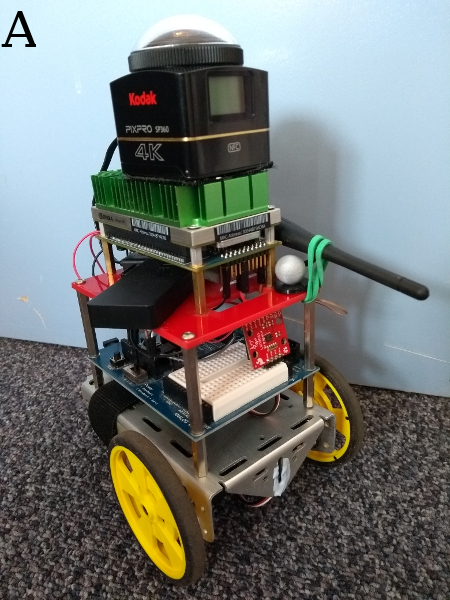
\includegraphics[width=2in]{figures/robot.jpg}
    \caption{Robot platform with onboard computation.}
    \label{fig:robot}
\end{figure}

\section{Methods}
As described above, at the heart of our algorithm is the use of a remembered view as a `visual compass' which can be used to recall the heading at which that view was stored. 
For an ant or wheeled robot that is constrained to move in the direction that is facing, the visual compass thus recalls the direction of movement when the view was stored. 
This process is implemented by rotating the current view and finding the most familiar direction either by inputting to the ANN encoding or, as a control, comparing iteratively to the set of training views. 
In the following sections we first describe the iterative algorithm followed by the Infomax ANN architecture.

\begin{figure}[t]
    \centering
    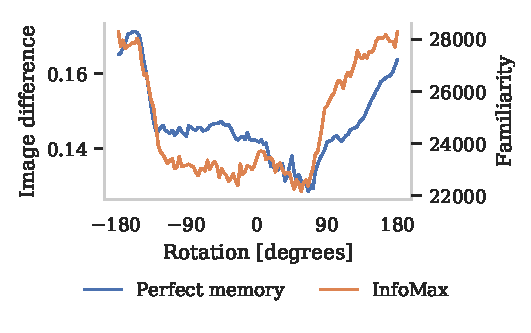
\includegraphics{figures/good_ridf.eps}
    \caption{Example Rotational Image Difference Function~(RIDF) from Perfect memory algorithm and Rotational Familiarity Function~(RFF) from InfoMax.}
    \label{fig:good_ridf}
\end{figure}

\subsection{RIDF and Perfect memory}
\label{sec:ridf_perfect_memory}
As a comparison to the Infomax ANN we describe in the next section, we also use a `perfect memory' version of the algorithm. 
In this variant, each rotated view is simply compared to all of the training views in turn. 
The best matching heading is then defined as the one with the lowest image difference, across all training views and rotations. 
The image difference can be calculated by various functions but, here we use the average absolute difference between each of the image pixels to calculate the Image Difference Function~(IDF): \todo{fix formula}
%
\begin{align}
    IDF(I(x,t),Ti(y,p)) = sqrt Sum Sum ()
\end{align}
%
where $I(x,t)$ and $Ti(y,p)$.\todo{finish} 
An Rotational Image Difference Function~(RIDF) is thus generated by varying theta\todo{there is no theta} though a range of angles and calculating the IDF at each rotation. 
Where there is a good match, there will be a minimum in the RIDF which defines the best matching direction. 
An example RIDF is shown in figure~\ref{fig:good_ridf} which has a clear minimum at the best matching heading of around \SI{60}{\degree}.
As the RIDF will also have minima at other matching headings, we can use this to analyse points where there has been a good or bad match to see if there is any aliasing.  

\begin{figure}[t]
    \begin{subfigure}[b]{\columnwidth}
        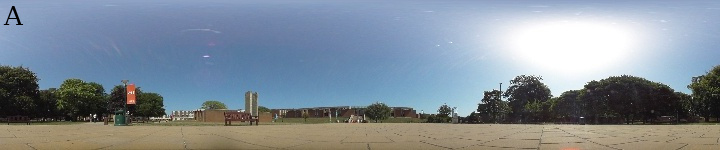
\includegraphics[width=\columnwidth]{figures/360_240.jpg}
        \caption{Unprocessed panoramic image}
    \end{subfigure}
    \begin{subfigure}[b]{\columnwidth}
        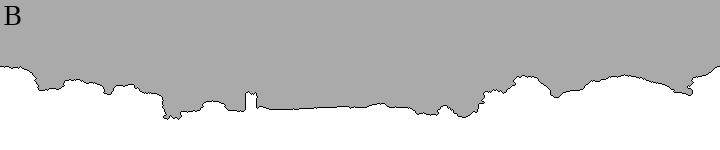
\includegraphics[width=\columnwidth]{figures/360_240_mask.png}
        \caption{Sky-segmented panoramic image}
    \end{subfigure}
    \caption{Example panoramic images from our database}
    \label{fig:database_images}
\end{figure}

\begin{figure*}[t]
    \centering
    \begin{subfigure}[t]{0.3\textwidth}
        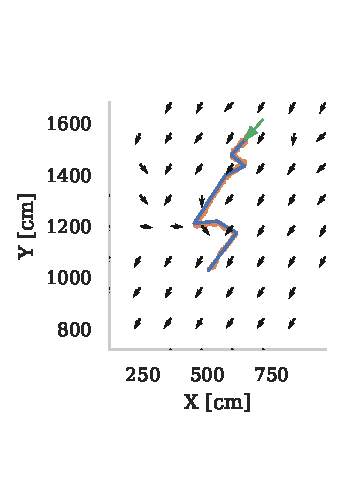
\includegraphics{figures/vector_field_route2_PerfectMemory_mask.eps}
        \caption{Simple route (route 2)}
        \label{fig:vector_fields/route2_perfect_memory_mask}
    \end{subfigure}
    \begin{subfigure}[t]{0.3\textwidth}
        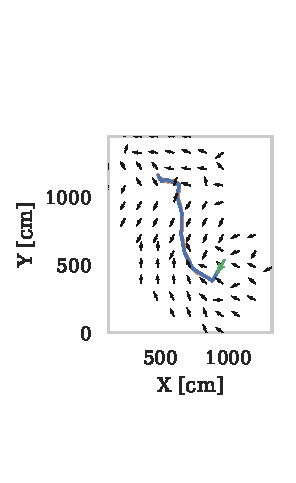
\includegraphics{figures/vector_field_route5_PerfectMemory_mask.eps}
        \caption{Longer route (route 5) where visual aliasing occurs in the middle section}
        \label{fig:vector_fields/route5_perfect_memory_mask}
    \end{subfigure}
    \begin{subfigure}[t]{0.3\textwidth}
        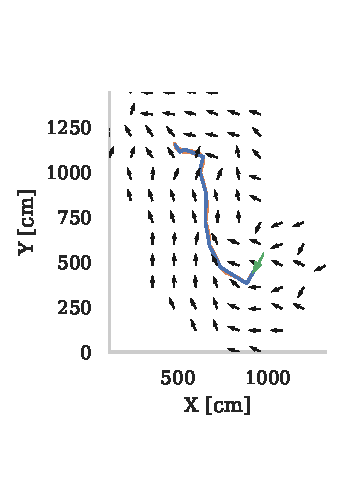
\includegraphics{figures/vector_field_route5_PerfectMemoryConstrained_mask.eps}
        \caption{By only considering rotated views within 90° of the route, visual aliasing problems can be avoided in route 5.}
        \label{fig:vector_fields/route5_perfect_memory_constrained_mask}
    \end{subfigure}
    
    \caption{Vector fields showing the directions an agent, trained on a route, would move at each point within 4m of the route using a Perfect Memory algorithm with the skyline extracted using the watershed algorithm. 
    Orange lines shows data from our camera-based tracking of the robot and blue lines show the version simplified using the Ramer-Douglas-Peucker algorithm~\citep{Ramer1972}.
    Green arrows indicate the position and direction the robot starts at.}
    \label{fig:vector_fields}
\end{figure*}

\subsection{Familiarity and Infomax}
\label{sec:familiarity_infomax}
In order to perform familiarity discrimination we chose to use a neural network model that was specifically designed to perform this task~\citep{Lulham2011}. 
The architecture consists of an input layer and a novelty layer with $tanh()$ activation functions. 
The number of input units is equal to the dimensionality of the input which in our case is $[120 \times 25]=3000$, the number of pixels in a down-sampled view of the world. 
The number of novelty units is arbitrary and here we follow \citet{Lulham2011} and use the same number of novelty units as inputs. 
We found that using as few as \num{200} novelty units can work well in many instances, but we do not explore this aspect of the problem as we were more interested in the behavioural consequences of a familiarity driven approach. 
The network is fully connected by feedforward connections $w_{ij}$. 
Weights are initialised randomly from a uniform distribution in the range $[-0.5,0.5]$ and then normalised so that the mean of the weights feeding into each novelty unit is \num{0} and the standard deviation is \num{1}. 
The network is then trained using the Infomax principle~\citep{Bell1995}, adjusting the weights so as to maximise the information that the novelty units provide about the input, by following the gradient of the mutual information. 
In our learning scheme, equation~\ref{eqn:infomax_learning} is used to perform gradient ascent using the natural gradient~\citep{Amari1998} of the mutual information over the weights~\citep{Lee1997} (use of the natural gradient avoids the computationally expensive calculation of the inverse of the entire weight matrix). 
Since two novelty units that are correlated carry the same information, adjusting weights to maximise information will tend to de-correlate the activities of the novelty units and the algorithm can thus be used to extract independent components from the training data~\citep{Lee1997}. 
We choose to use this approach mainly because it only requires a single pass through the data, meaning that each view is experienced just once and then discarded. 
While, with a limited amount of data, the algorithm is unlikely to converge to a particularly good set of independent components, it is enough that the components that are extracted provide a more suitable decomposition of the training data than of an arbitrary input.
During learning the activation of each of the $M$ novelty units $h_{i}$ is computed as:
%
\begin{align}
    h_{i}=\sum\limits_{j=1}^N w_{ij}x_{j}   \label{eqn:infomax_activation}
\end{align}
%
where $x_{i}$ is the value of the $ith$ input and $N$ is the number of input units. 
The output $y_{i}$ of the novelty units is then given by:
%
\begin{align}
    y_{i}=tanh(h_{i})   \label{eqn:infomax_output}
\end{align}
%
The weights are then adjusted using the following learning rule: 
%
\begin{align}
    \Delta w_{ij}=\frac{\eta}{N} \Bigl( w_{ij} - (y_{i} + h_{i}) \sum\limits_{k=1}^N h_{k}w_{kj} \Bigr)   \label{eqn:infomax_learning}
\end{align}
%
where $\eta$ is the learning rate and is set as \num{0.01} for this paper. 
Finally, the response of the network to the presentation of an unseen N-dimensional input $\vec{x}$ is computed as
%
\begin{align}
    d(\vec{x})=\sum\limits_{i=1}^M |h_{i}|     \label{eqn:infomax_response}
\end{align}
%
where $||$ denotes the absolute value. 
The network response could be viewed as an output layer but, as it is a function of the activations of the novelty units, we follow \citet{Lulham2011} and do not represent it with another layer. 
As noted above, in this paper, we set $M=N$ and the network is trained with each training view presented just once to the network in the order in which it is experienced in training. 
\citet{Lulham2011} use $d(\vec{x})$ together with a threshold that must be determined empirically to determine whether the input is novel or familiar. 
For our purposes it is not necessary to determine a threshold as we only need to choose the most familiar input from a limited number of possibilities i.e. the views experienced during a single scan of the environment.

The difference between the way an image difference function and a neural network trained using an Infomax principle represent familiarity will be subtle. 
In essence, the difference is manifest in the way the information is stored. 
For image differences, each stored view defines a single point in an N-dimensional space, with N equal to the dimension of the images ($N = 120 \times 25 = 3000$) and the image difference function gives the squared Euclidean distance of an input image from one of these stored points. 
This requires that all of the views are stored, meaning that memory load increases proportional to the number of views experienced. 
The Infomax approach instead decomposes each view into a fixed number of components (determined by the number of hidden units in the network) which remains fixed, independent of the number of views experienced. 
Therefore, the Infomax measure is more abstract and reflects whether a test input is well described in terms of the learned components that the hidden units represent. 
However, by decomposing the input in this way, it is possible to compress redundant data resulting in more efficient memory storage.


\subsection{Robot platform}
\label{sec:robot_platform}
In this work we use the robot platform developed by \citet{Domcsek2018} shown in figure~\ref{fig:robot}.
This robot is based on a Parallax `Shield-Bot' chassis~\citep{ParallaxInc}, with a Jetson TX1 embedded computer~\citep{NVIDIACorporation2016} mounted on top for additional onboard computation and additional batteries mounted underneath. 
The Jetson TX1 is connected via USB to a Kodak PixPro SP360 4K camera~\citep{JKImagingLtd}, mounted on top of the robot connected which provides panoramic visual input.

\subsection{Image database}
\label{sec:image_database}
Using a Kodak PixPro SP360 4K panoramic camera~\citep{JKImagingLtd}, we recorded \num{195} images of the ‘Library Square’ at the University of Sussex. 
These were taken on a \SI{1.2}{\metre} grid, aligned with the slabs the square is paved with.
As well as this reference grid of images, we also recorded videos from the same camera mounted on the mobile robot described in the previous section, as we manually drove it along six routes of varying lengths and tortuosity across the square. 
We tracked the robot by using the Discriminative Correlation Filter Tracker with Channel and Spatial Reliability~\citep{Lukezic2018} implementation provided by OpenCV~\citep{OpenCV} to extract the position of the robot over time from video captured by a tripod-mounted camera. 
Finally, we used OpenCV to apply a perspective transform to the positions extracted by the tracker and married these final positions with the video frames captured by the robot. 
\citet{Stone2014} showed that sky-segmented, binary images can be used for robust visual navigation and, while our robot does not have a suitable UV camera, by using the watershed segmentation algorithm~\citep{Beucher1979} with markers placed at the top and bottom of each image, we obtained automatically sky-segmented versions of all of the images in our dataset.
Figure~\ref{fig:database_images} shows some example images from this database.

\begin{figure}[t]
    \begin{subfigure}[b]{\columnwidth}
        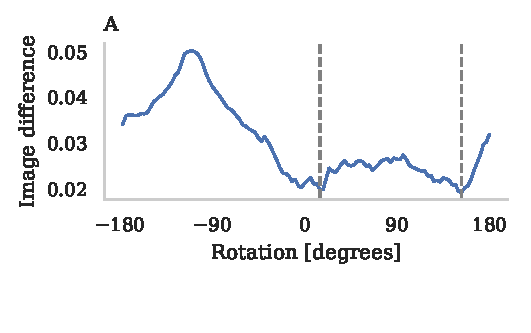
\includegraphics[width=\columnwidth]{figures/alias_ridf.eps}
        \caption{Rotational Image Difference function}
        \label{fig:aliasing/ridf}
    \end{subfigure}
    
    \begin{subfigure}[b]{\columnwidth}
        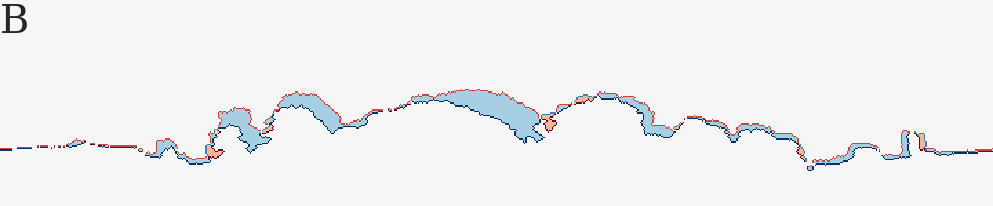
\includegraphics[width=\columnwidth]{figures/image_diff_bad.png}
        \caption{Difference image with visual aliased route image}
        \label{fig:aliasing/image_diff_bad}
    \end{subfigure}
    
    \begin{subfigure}[b]{\columnwidth}
        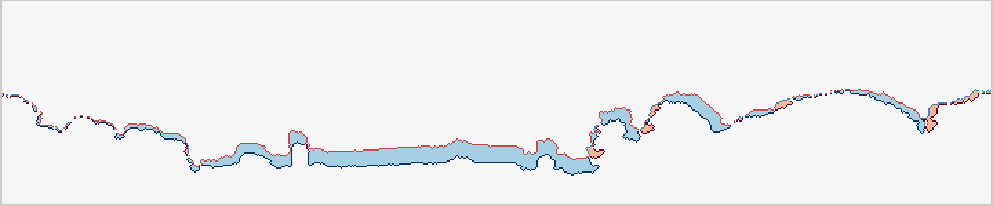
\includegraphics[width=\columnwidth]{figures/image_diff_good.png}
        \caption{Difference image with correct route image}
        \label{fig:aliasing/image_diff_good}
    \end{subfigure}
    \caption{Analysis of aliasing shown in figure~\ref{fig:vector_fields/route5_perfect_memory_mask}.
    Using grid image taken at (\SI{600}{\metre}, \SI{720}{\metre}).
    All images were pre-processed using watershed segmentation algorithm.}
    \label{fig:aliasing}
\end{figure}

\begin{figure*}[t]
    \centering
    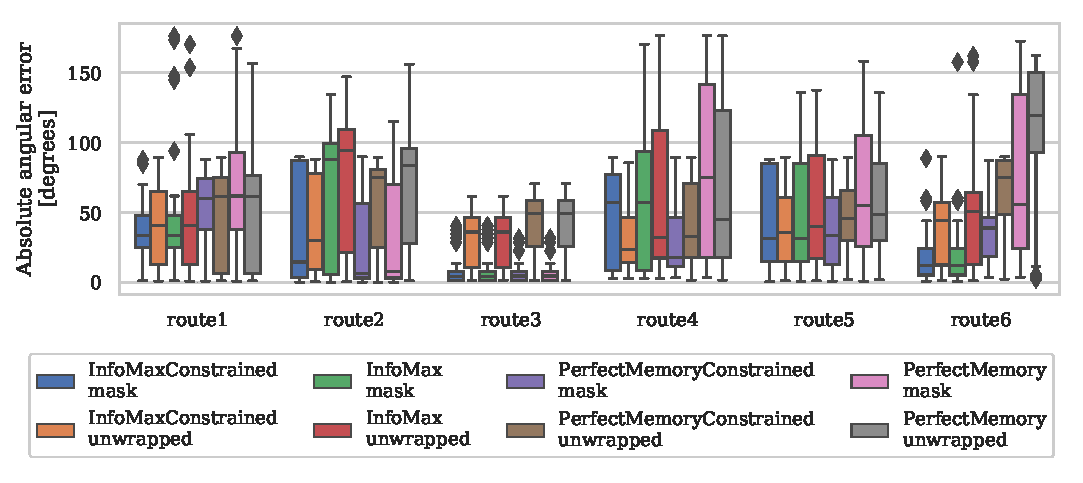
\includegraphics{figures/route_benchmark.eps}
    \caption{Performance of different algorithms on each of the 6 routes. \todo{decide on consistent names for routes}}
    \label{fig:route_benchmark}
\end{figure*}

\begin{figure}[t]
    \begin{subfigure}[b]{\columnwidth}
        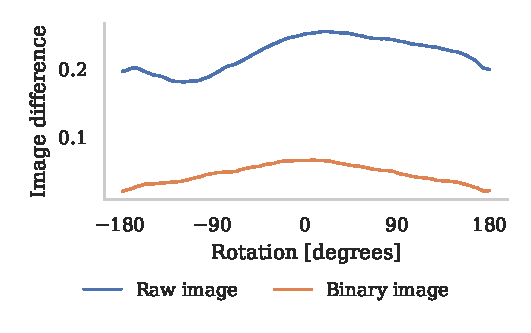
\includegraphics[width=\columnwidth]{figures/route3_ridf.eps}
        \caption{Rotational Image Difference function}
        \label{fig:light_level/ridf}
    \end{subfigure}
    
    \begin{subfigure}[b]{\columnwidth}
        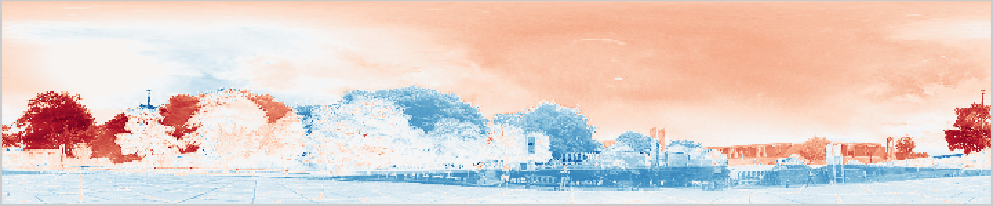
\includegraphics[width=\columnwidth]{figures/route3_unwrapped_image_diff.png}
        \caption{Difference image based on raw input images}
        \label{fig:light_level/raw_image_diff}
    \end{subfigure}
    
    \begin{subfigure}[b]{\columnwidth}
        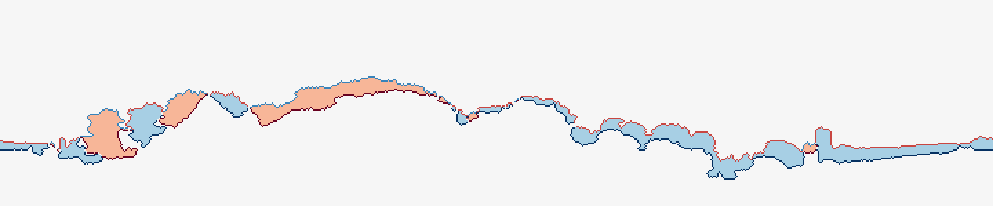
\includegraphics[width=\columnwidth]{figures/route3_mask_image_diff.png}
        \caption{Difference image based on sky-segmented input images}
        \label{fig:light_level/sky_segmented_image_diff}
    \end{subfigure}
    \caption{Analysis of poor performance on route 3 when using raw input images.
    Using grid image taken at (\SI{480}{\metre}, \SI{720}{\metre}).}
    \label{fig:light_level}
\end{figure}

\section{Results}
\subsection{Image database}
We trained both the InfoMax and Perfect Memory algorithms on the images taken along the six routes in our dataset and then used them to find the direction a robot would move when placed at each grid point within \SI{4}{\metre} of the trained route. 
Figure~\ref{fig:vector_fields} shows some example vector fields obtained by plotting this direction at each of the chosen grid locations when using the Perfect Memory algorithm described in section~\ref{sec:ridf_perfect_memory} with the watershed segmentation-based preprocessing discussed in section~\ref{sec:image_database}. 
While the vector field suggests that the route shown in Figure~\ref{fig:vector_fields/route2_perfect_memory_mask} would be recapitulated successfully, in the middle section of the route shown in Figure~\ref{fig:vector_fields/route5_perfect_memory_mask}, errors occur.
Figure~\ref{fig:aliasing/ridf} shows a RIDF taken at one of the problematic locations on this route \todo{mark grid and add arrows showing aliases} (\SI{600}{\metre}, \SI{720}{\metre}) and it is clear that, as well as the local minima representing the correct heading at \SI{15}{\degree}, there is an additional, slightly lower local minima at \SI{153}{\degree} which is overriding the correct choice.
Figures~\ref{fig:aliasing/image_diff_bad}~and~\ref{fig:aliasing/image_diff_good} show the per-pixel differences between the two route images and the rotated versions of the grid image which correspond with these minima and this makes the cause of the problem become clear.
Although the \emph{shapes} of the skylines in figure~\ref{fig:aliasing/image_diff_good} are clearly more similar than those in figure~\ref{fig:aliasing/image_diff_bad}, there is a vertical offset -- probably caused by camera shake -- which introduces a large difference between the two images.

However, if we were recapitulating the route using a real robot, these false-positive matches could be eliminated and computation could be saved by simply \emph{not} scanning the full \SI{\pm 180}{\degree}. 
We simulated the effect of this modified algorithm using our database of images by simplifying each route using the Ramer-Douglas-Peucker algorithm~\citep{Ramer1972} and calculating the direction of each of the resultant segments.
Using these headings, we can then ignore matches that would involve heading more than \SI{\pm 90}{\degree} away from the direction of the nearest section of the route.
Figure~\ref{fig:vector_fields/route5_perfect_memory_constrained_mask} shows that this step solves the aliasing problems in this particular case and figure~\ref{fig:route_benchmark} confirms that, infact, this step improves performance across all algorithms and routes.
Furthermore, figure~\ref{fig:route_benchmark} also shows that, when using the Perfect Memory algorithm, sky-segmentation improves performance for almost all routes.
This is particularly noticeable on route 3 (a straight line) where, when using sky-segmented input images, all of the algorithms reconstruct the direction of the route with a very small median error of around \SI{4}{\degree} but, when using unprocessed input images, this increases to around \SI{40}{\degree}.
Figure~\ref{fig:light_level/ridf} shows that, unlike the situation explored earlier in this section, this is not an aliasing problem as there is only a single minima present in each RIDF.
However, the magnitude of the average image differences between the raw images is much larger than that between the sky-segmented images and the minima is located at the incorrect location.
The difference images shown in figures~\ref{fig:light_level/raw_image_diff}~and~\ref{fig:light_level/sky_segmented_image_diff} suggest that the incorrect position of the minima when comparing the raw images is likely to be due to the large differences in the sky portion of the image due to clouds and the images having been recorded at a different time of day.

This improvement is less significant when using the InfoMax algorithm but, 
\todo{explore case where InfoMax succeeds when PM doesn't}

\begin{figure}[t]
    \centering
    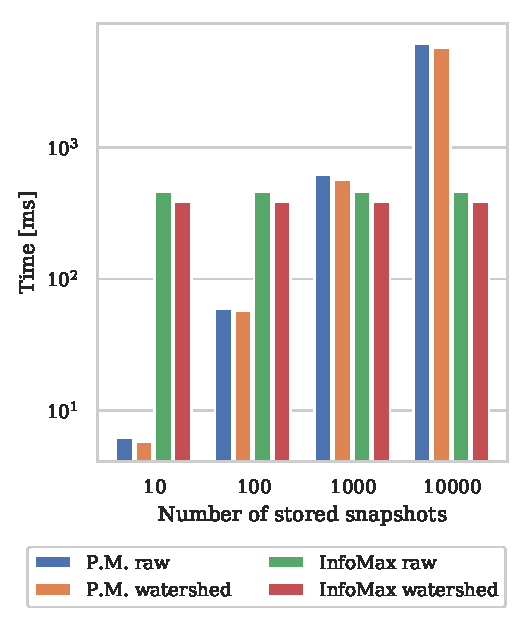
\includegraphics{figures/jetson_test_performance.eps}
    \caption{Performance of visual navigation algorithms running on Jetson TX1. 
    Reported times are measured using \lstinline{std::chrono::high_resolution_clock} and average is taken over \num{100} images.}
    \label{fig:jetson_test_performance}
\end{figure}

\subsection{Computational cost of algorithm}
In the previous section, we showed that the algorithms described in sections~\ref{sec:ridf_perfect_memory}~and~\ref{sec:familiarity_infomax} are capable of robustly extracting heading direction in outdoor scenes. 
However, in order to deploy these algorithms on a real robot with constrained on board processing, their performance is important. 

\begin{figure}[t]
    \centering
    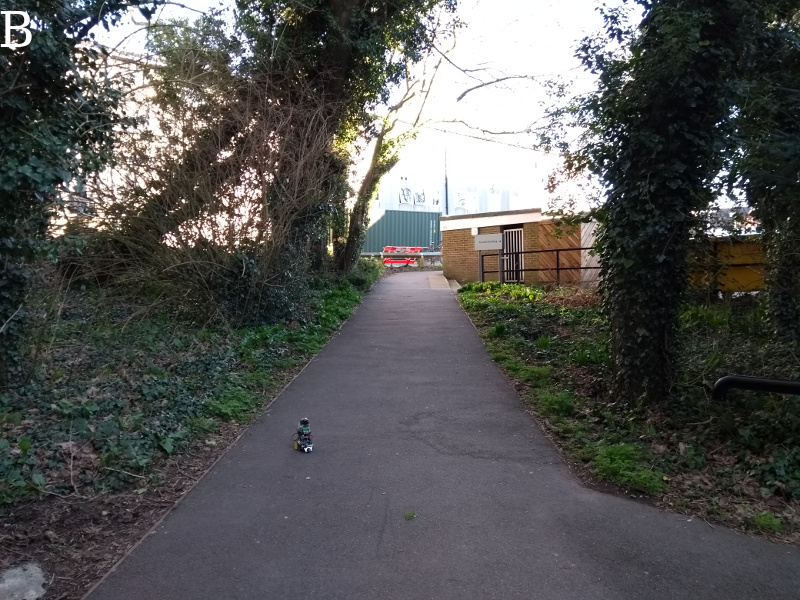
\includegraphics[width=2in]{figures/robot_environment.jpg}
    \caption{Environment used for robot testing.}
    \label{fig:robot_environment}
\end{figure}

\begin{figure}[t]
    \centering
    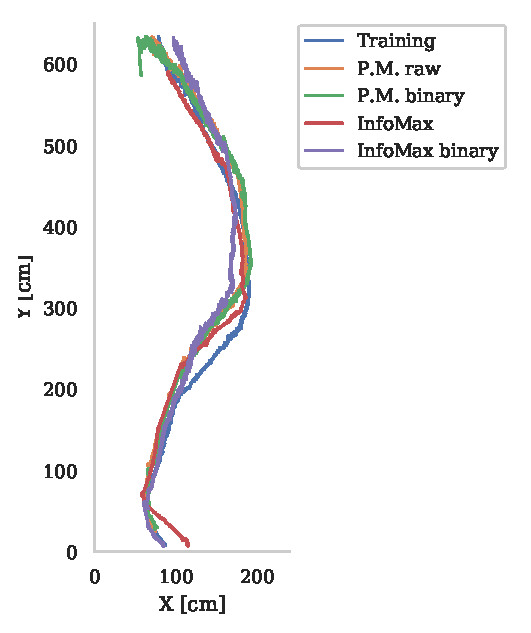
\includegraphics{figures/robot_paths.eps}
    \caption{Reconstructed paths of autonomous robot during training and testing using each algorithm.}
    \label{fig:robot_paths}
\end{figure}

\subsection{Autonomous robot}
Using the implementations of InfoMax and the Perfect Memory algorithms from our Brains-on-Board Robotics \todo{ref} library, we built a simple application which can recapitulate learned routes on the robot described in section~\ref{sec:robot_platform} by running the following simple algorithm every \SI{500}{\milli\second} (based on the performance for 1000 images established in the previous section):
%
\begin{enumerate}
    \item Capture and unwrap a panoramic image.
    \item Perform one of the image processing steps described in section~\ref{sec:image_database}.
    \item Using either the InfoMax or Perfect Memory algorithm, calculate the familiarity with the processed image ‘in-silico’ when rotated through \SI{\pm 90}{\degree}°.
    \item Find the orientation with the highest familiarity and, if it is within \SI{4}{\degree} \todo{CHECK}, start driving forwards. Otherwise, start turning in the correct direction to align with the image.
\end{enumerate}
%
In order to compare the performance of the navigation algorithms and image processing steps described in sections~\ref{sec:ridf_perfect_memory},~\ref{sec:familiarity_infomax}~and~\ref{sec:image_database} running on the robot, we first manually drove the robot along a sinuous route through the wooded area shown in figure~\ref{fig:robot_environment}, recording training images every \SI{100}{\milli\second}\todo{check}.
We then trained each of the navigation algorithms on the resultant dataset of \num{455} images and allowed the robot to recapitulate the path using the procedure described above.
Throughout this training and testing process, we used the method described in section~\ref{sec:image_database} to track the robot, resulting in the data shown in figure~\ref{fig:robot_paths}.
The robot was able to successfully recapitulate the training path using each of the navigation and image processing algorithms with little difference in performance immediately apparent in figure~\ref{fig:robot_paths}.
We confirmed this by calculating the shortest distance to the training path at each location along each recapitulated path and found that, in this environment, there was no significant difference between the performance of the different algorithms and overall the mean of the distance between the training and recapitulated paths was \SI{9}{\centi\metre}, with a standard deviation of \SI{8}{\centi\metre}.
\todo{same time of day -- differences between algorithms less significant}

\section{Discussion}
\begin{itemize}
    \item how/why SLAM is the obvious alternative
    \item General limitations of monocular SLAM
\end{itemize}
Typically, visual SLAM implementations extract features such as SURF or SIFT which require several hundreds of milliseconds to extract per frame~\citep{Bay2006}. 
This makes such implementations impractical to use in real-time, especially on constrained mobile platforms. 
However, more recent SLAM implementations such as FLaME~\citep{Greene2017} have been shown to run on autonomous quadrotors in only around \SI{10}{\milli\second} per frame. 
While this is significantly faster than our current InfoMax implementation, \citet{Greene2017} were using a much more powerful Intel CPU on their quadrotor which \citet{Biddulph2018} measured as being $5\times$ faster than a Jetson TX1. 
Additionally, we used $120 \times 25$ pixel images for all of the work presented in this paper but, when \citet{Baddeley2012} first demonstrated InfoMax for visual navigation, they used input images with around half this number of pixels~($90\times 17$).
Equation~\ref{eqn:infomax_response} can be implemented as a matrix-vector product -- the computational cost of which scales quadratically with $N$.
Therefore, using input images with half the number of pixels would quarter the time taken to evaluate equation~\ref{eqn:infomax_response}.
Furthermore, while our InfoMax implementation uses OpenMP~\todo{citation} to take advantage of the the Jetson TX1's four CPU cores, it does not utilise the \num{256} core GPU present on the Jetson TX1.
Initial experiments using the cuBLAS~\citep{NVIDIACorporation2007} GPU-accelerated linear algebra library suggest that equation~\ref{eqn:infomax_response} could be evaluated in around \SI{100}{\milli\second} for $120 \times 25$ pixel images -- a $5 \times$ speedup over our current implementation.

\section{Conclusions}
\begin{itemize}
    \item When used in outdoor environments, the performance of insect-inspired visual homing algorithms can be much improved by applying automatic sky-segmentation to the input images. This helps make these algorithms more robust to different lighting and weather conditions.
    \item InfoMax - better?
\end{itemize}

\section{Acknowledgements}
This work was funded by the EPSRC (Brains on Board project, grant number EP/P006094/1).
We would also like to thank Daniil Sakhapov for his work collecting the `Library Square' database of images, Alex Dewar for developing the BoB robotics framework and Norbert Domcsek for assisting with the data collection for this paper. 

\footnotesize
\bibliographystyle{apalike}
\bibliography{alife} % replace by the name of your .bib file


\end{document}
